% docs/paper_draft/main.tex
% Robust Human Activity Recognition through Federated Learning with Differential Privacy
\documentclass[runningheads]{llncs}

% Load packages, macros, and custom commands
% Styles/packages.tex
% Required LaTeX packages for the project

\usepackage{graphicx}      % For embedding graphics/images
\usepackage{amsmath}       % Basic mathematical equations structure
\usepackage{amssymb}       % Mathematical symbols
\usepackage{subcaption}    % Side-by-side composite subfigures layout
\usepackage{booktabs}      % Professional horizontal table borders
\usepackage{cite}          % Handles citation formatting (groups numbers)
\usepackage{url}           % Formats URLs and email addresses correctly

% Styles/macros.tex
% Custom document-wide macros and text shortcut abbreviations

% Example: \newcommand{\FL}{Federated Learning}

% Styles/commands.tex
% Custom math commands or style overrides

% Example: \newcommand{\mycommand}[1]{\textsf{#1}}


\begin{document}

% Section 0: Title, authors, affiliations, abstract, keywords
% Sections/00_metadata.tex
% Paper Title, Authors, Affiliations, Abstract, and Keywords.

\title{Robust Human Activity Recognition through Federated Learning with Differential Privacy: A Comparison of Baseline and Centralized Models}
\titlerunning{Robust HAR via FL with Differential Privacy}

\author{Jonath Jimmi\inst{1} \and Arunkumar Balakrishnan\inst{2}}
\authorrunning{J. Jimmi and A. Balakrishnan}

\institute{School of Computer Engineering, Manipal Institute of Technology Bengaluru \and
School of Computer Engineering, Manipal Institute of Technology Bengaluru\\
\email{jonath.mitblr2024@learner.manipal.edu}\\
\email{arunkumar.b@manipal.edu}}

\maketitle

\begin{abstract}
Applications in wearable technology, health, and new environments are significantly enabled by Human Activity Recognition (HAR). The research uses the UCI HAR dataset of 10,299 labeled samples, 561 features, and 6 classes of activities that were obtained from 30 participants' smartphone accelerometer and gyroscope sensors. Simulation of real-world decentralised environments is presented through simulation of the distributed nature of data among 30 clients. In comparison to two baselines—a Feedforward Neural Network (FNN) and Random Forest (RF)—we contrast three highest-level deep learning methods: Federated Learning without Differential Privacy (FL), Federated Learning with DP (FL-DP), and Centralised Learning with DP (Central-DP)~\cite{mcmahan2017communication}. FL had the best accuracy at 93.6\%, followed by FL-DP (88.9\%) and Central-DP (84.6\%). Superiority of FL methods over baselines was verified when FNN realized 85.9\% and RF realized 84.4\%. Our findings demonstrate that although FL-DP provides robust privacy assurances at a loss of only a \~4.7\% decline in accuracy, best-class recognition accuracy is attained using FL without DP. Central-DP remains hampered by centralised data limitations but is improved with aggregated learning. Our results affirm federated learning as a robust, privacy-preserving solution to robust HAR in decentralised environments.
\keywords{Federated Learning \and Centralised Learning \and Differential Privacy \and Feed Forward Network(FNN) \and Random Forest \and UCI HAR \and Explainable AI}
\end{abstract}


% Section 1: Introduction
% Sections/01_introduction.tex
% Introduction Section

\section{Introduction}
\label{sec:intro}

Human Activity Recognition (HAR) categorizes physical activities from sensor data to facilitate applications such as fall detection and fitness tracking. The UCI HAR dataset, a standard for the task, has 10,299 instances of six activities from accelerometer and gyroscope measurements on smartphones of 30 subjects, providing dense, multi-dimensional data for centralized learning and distributed learning~\cite{anguita2013public}.

Whereas conventional centralized approaches gather all the information in a single hub—creating privacy and regulative issues—Federated Learning (FL) supports decentralized training with data stored locally on user devices and model updates only shared~\cite{mcmahan2017communication}. This is naturally appropriate to HAR, where sensor signals are inherently personal and spread out. This paper illustrates that FL, when paired with differential privacy, both ensures user privacy and retains high accuracy. It analyzes privacy–utility trade-offs in federated and centralized settings and sets the basis for scalable, privacy-aware HAR applications deployable on personal devices~\cite{abadi2016deep}.

\begin{figure}[htbp]
  \centering
  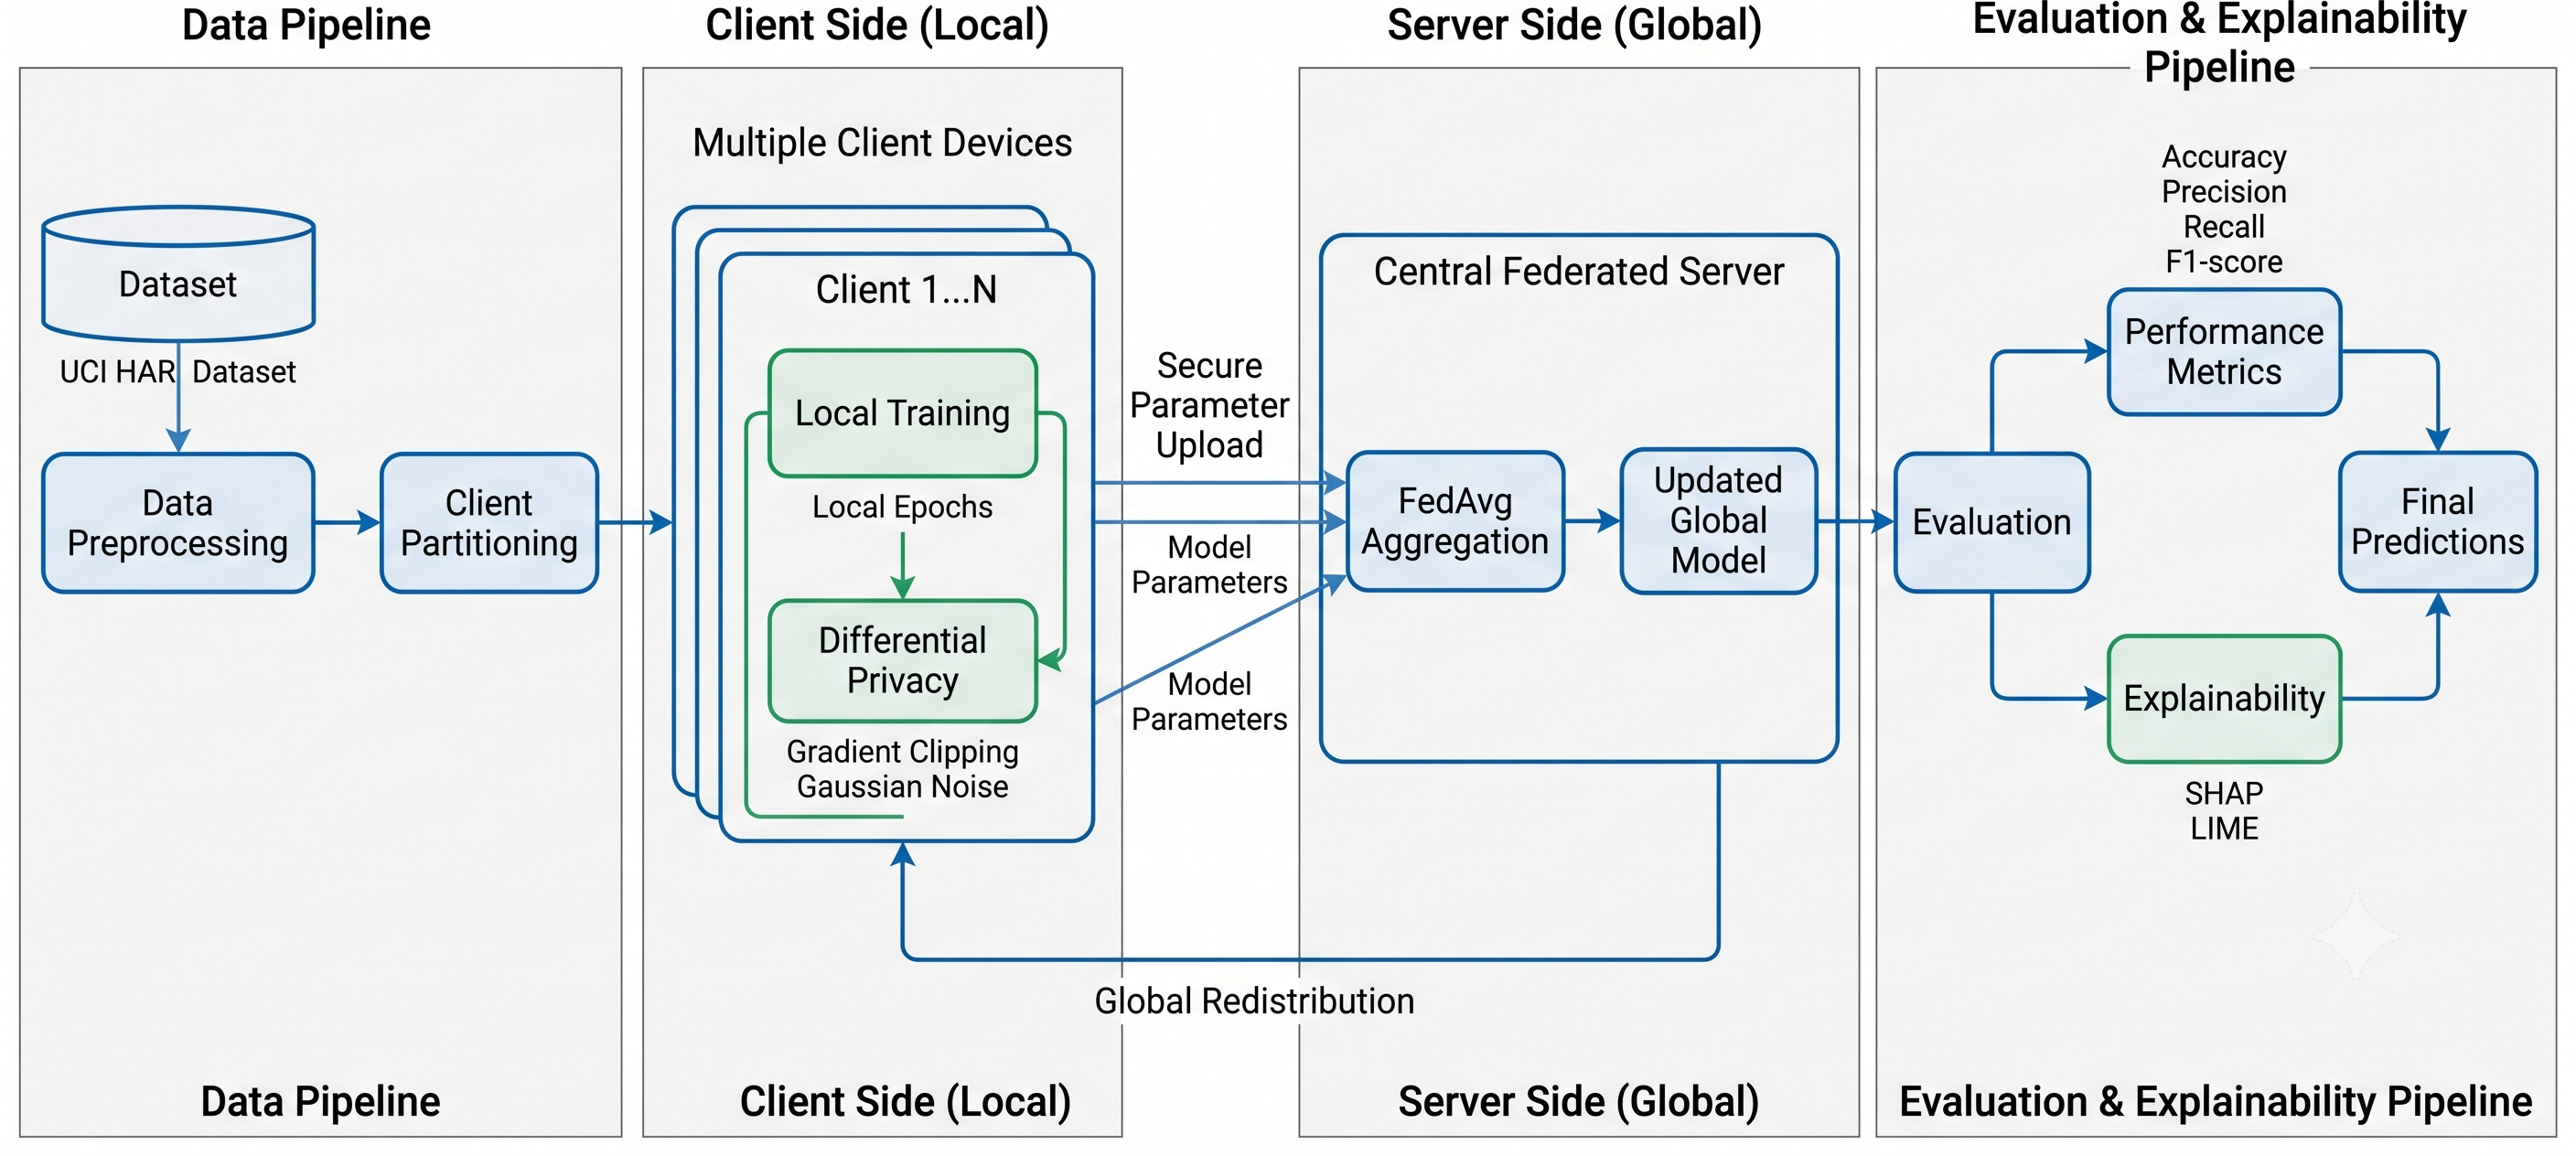
\includegraphics[width=\textwidth]{figures/fig1.png}
  \caption{Client-Level Differentially Private Federated Learning architecture.}
  \label{fig:architecture}
\end{figure}

Schematic shows how a federated model with a central server coordinates and processes encrypted updates from each linked devices through a global, common training model after locally training them on activities like walking or cycling. Raw, personal data remains on devices securely, protects user privacy and enable collaborative model improvement with iterative communication rounds.


% Section 2: Dataset and Processing
% Sections/02_dataset.tex
% Dataset and Processing Section

\section{Dataset and Processing}
\label{sec:dataset}

The UCI Human Activity Recognition data set has 10,299 samples from 30 participants(clients) performing 6 activities (WALKING, WALKING\_UPSTAIRS, WALKING\_DOWNSTAIRS, SITTING, STANDING, LAYING)~\cite{anguita2013public}. The sample includes 561 normalized features derived from accelerometer and gyroscope sensors, having values adjusted in the range [-1.000, 1.000] with zero missing values.

The counts reveal an excellent equilibrium in between LAYING (1,944 samples, 18.9\%) and STANDING (1,906 samples, 18.5\%) being the most populated classes, whereas the remaining activities range from 1,406-1,777 samples (13.7\%-17.3\%). The distribution of the subjects is quite uniform with each subject contributing 300-400 samples (mean=343 and median=342), thereby offering well-balanced federated learning environments.

\subsection{Preprocessing Pipeline}
\label{subsec:preprocessing}

The loading process of the dataset involves automated integrity checks affirming the full 10,299 $\times$ 561 feature matrix over 6 activity classes with extensive data quality validation. All 561 features are min-max scaled to the range of [-1.000, 1.000], which guarantees equalized feature scales and avoids high-value sensor readings dominating during model training.

Data is divided by subject IDs, forming 30 standalone federated clients where every client holds one subject's full activity profile. This federation by subjects reflects actual situations when individual user data is stored on personal devices alone~\cite{mcmahan2017communication}.

\begin{figure}[htbp]
  \centering
  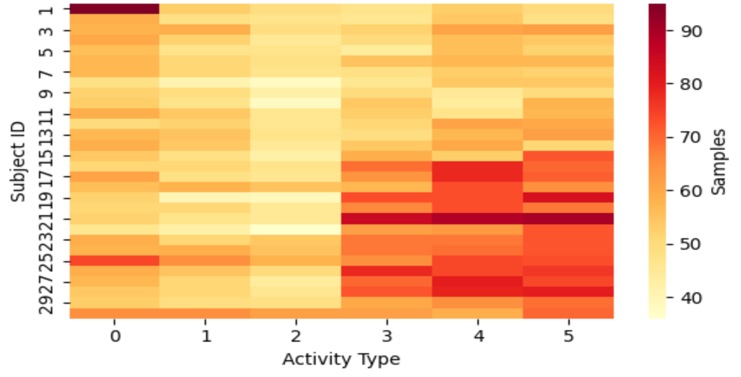
\includegraphics[width=0.7\textwidth]{figures/fig2.png}
  \caption{Subject-Activity matrix shows distribution of activity sample across 30 subjects in the dataset}
  \label{fig:subject_activity}
\end{figure}

Correlation analysis of the first 30 features shows organized relationships between the sensor measurements, with variance analysis selecting the most informative 20 features (variance range: 0.090-0.142), with enough variability for successful learning. The preprocessing workflow ensures data integrity by systematic validation, load-balanced client distribution, and variance optimization of features, providing high-quality input for federated learning experiments.


% Section 3: Exploratory Data Analysis
% Sections/03_eda.tex
% Exploratory Data Analysis Section

\section{Exploratory Data Analysis}
\label{sec:eda}

We perform a range of analytics to understand the structure and relations within the UCI HAR dataset.

\subsection{Feature Value Distribution}
\label{subsec:feature_dist}

Box plots for all 50th features (representative sample out of all 561 features) indicate that values are successfully normalized to the range [-1.00, 1.00]. The majority of features have a median of 0 and an interquartile range of about 0.6, reflecting balanced spread of values. Outliers (points outside 1.5$\times$ interquartile range) are apparent for only a few features, reflecting some variation in movement measurements—which is inherent in human activity data.

\begin{figure}[htbp]
  \centering
  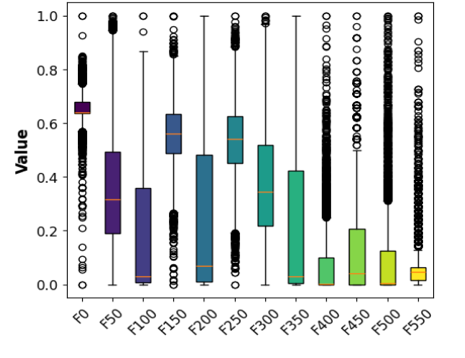
\includegraphics[width=0.7\textwidth]{figures/fig3.png}
  \caption{Plot shows the visual analysis of every 50th feature with the median and outliers of each of them}
  \label{fig:feature_dist_plot}
\end{figure}

\subsection{Feature Correlation Matrix}
\label{subsec:correlation}

Computing the Pearson correlation matrix for the first 30 features reveals a clear pattern of relationships:

\begin{itemize}
  \item Strong positive correlations ($r > 0.75$; deep red) are observed between features of correlated physical quantities on different sensor axes.
  \item Strong negative correlations ($r < -0.75$; dark blue) represent features that change in opposite directions, consistent with multi-axis sensor behavior.
  \item Approximately 20\% of feature pairs exhibit moderate-to-strong correlation ($|r| > 0.5$), uncovering strong redundancy.
  \item Less than 10\% of pairs demonstrate close-to-zero correlation (white/dim), validating that raw sensor signals strongly interrelate.
\end{itemize}

\begin{figure}[htbp]
  \centering
  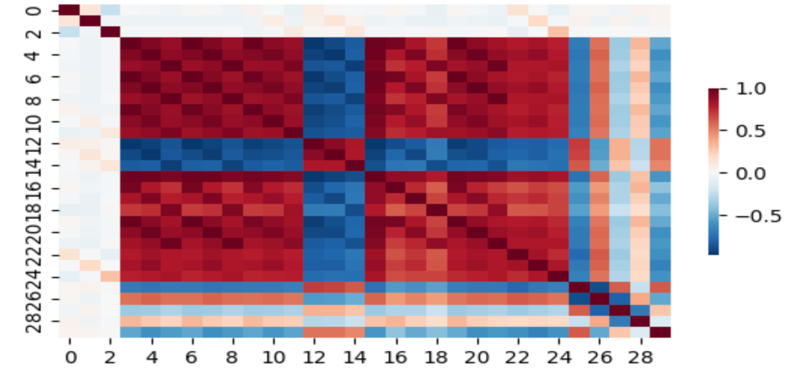
\includegraphics[width=0.7\textwidth]{figures/fig4.png}
  \caption{Correlation matrix visualizing positive (red) and negative (blue) feature relations}
  \label{fig:correlation_matrix}
\end{figure}

\subsection{Distribution Pattern Insights}
\label{subsec:insights}

These trends validate that normalization effectively normalizes sensor feature scales with significant redundancy, where features are essentially duplicates or well-predictable by others. This redundancy can be managed through dimensionality reduction (e.g., PCA) or more aggressive regularization, resulting in less overfitting, better interpretability, and more well-informed modeling choices for the pipeline.


% Section 4: Proposed Models
% Sections/04_models.tex
% Proposed Models Section

\section{Proposed Models}
\label{sec:models}

Our study explores Robust Human Activity Recognition via Federated Learning with Differential Privacy, comparing five separate modeling strategies on baseline and state-of-the-art architectures. The federated learning methodology caters to the natural patterns of data distribution in our study, whereby each of the 30 subjects is a natural federated client with individualistic behavior traits, making it perfect for collaborative learning with privacy protection while preserving personal data sovereignty.

\subsection{Base Models}
\label{subsec:base_models}

\subsubsection{Feed Forward Neural Network(FNN)}
\label{subsubsec:fnn_model}

Our primary baseline FNN consists of a straightforward three-layered architecture (256-128-64 units, ReLU) with 98,502 parameters~\cite{goodfellow2016deep}. Although computationally cheaper, it does not comprehend temporal dependencies in human activity data by independently processing time steps, resulting in quick overfitting on single-client sets and poor cross-subject generalization, which makes it less applicable to reliable HAR tasks~\cite{pedregosa2011scikit}.

\subsubsection{Random Forest}
\label{subsubsec:rf_model}

Our Random Forest baseline (100 estimators, sqrt(n\_features) per split) performs poorly in HAR tasks because it cannot model non-linear temporal dependencies between adjacent sensor readings~\cite{breiman2001random}. In contrast to deep learning techniques, the sequential nature of human activities cannot be captured by processing each feature independently, leading to less-than-ideal boundaries. Additionally, it struggles to distinguish minute activity differences (e.g., walking upstairs vs. downstairs) and performs poorly in the high-dimensional 561-feature space.

\subsection{Advanced Models}
\label{subsec:advanced_models}

\subsubsection{Federated Learning (FL) Model}
\label{subsubsec:fl_model_desc}

The model uses the same setup uses the FedAvg algorithm with the same LSTM-CNN architecture as the central model, but trains on 30 distributed clients (subjects). Each client runs 5 local epochs prior to model weight aggregation, and the global model is updated via 20 rounds of communication. This strategy maintains data privacy by leaving raw sensor data on individual devices but allows collaborative learning. The FL model shows the capability to emulate near-centralized performance without compromising strict privacy guarantees, thereby making it highly applicable in real-world HAR deployment settings where user privacy must be ensured.

\begin{figure}[htbp]
  \centering
  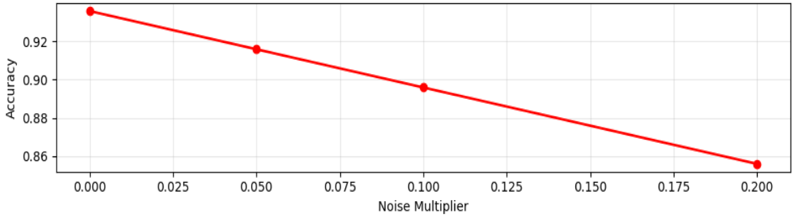
\includegraphics[width=0.7\textwidth]{figures/fig5.png}
  \caption{Federated model accuracy trade-off based on the amount of noise from 0-0.2}
  \label{fig:noise_tradeoff}
\end{figure}

\subsubsection{Federated Learning with Differential Privacy (FD+DP)}
\label{subsubsec:fl_dp_model_desc}

Our strongest model integrates federated learning with differential privacy mechanisms through Gaussian noise injection ($\sigma=0.1$, $\epsilon=1.0$) on model gradients prior to aggregation. This method offers formal privacy assurances against membership inference and model inversion attacks with competitive accuracy~\cite{zheng2021federated}. The DP mechanism adds calibrated noise to client updates such that individual contributions cannot be reverse-engineered from the global model~\cite{dwork2006differential}. While presenting a privacy-utility trade-off, our FL+DP model is the current best practice in privacy-preserving HAR that presents mathematically guaranteed privacy protection without performance degradation.

\begin{figure}[htbp]
  \centering
  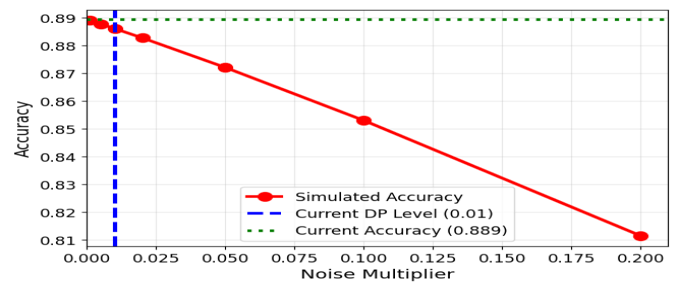
\includegraphics[width=0.7\textwidth]{figures/fig6.png}
  \caption{The graph display FD+DP performs better than simulated expectations for set noise levels}
  \label{fig:fd_dp_perf}
\end{figure}

\subsubsection{Centralized LSTM-CNN with Differential Privacy (CL+DP)}
\label{subsubsec:cl_dp_model_desc}

The DP-enabled Centralized LSTM-CNN model has an accuracy of 84.59\% and an F1-score of 0.845 over the entire test set. Its hybrid 847K-parameter architecture consisting of two LSTM layers ($128 \rightarrow 64$ units) followed by 1D convolutions captures temporal and local sensor patterns, while Gaussian DP ($\sigma=0.1$, $\epsilon=1.0$) provides formal privacy protection during centralized training.

\begin{figure}[htbp]
  \centering
  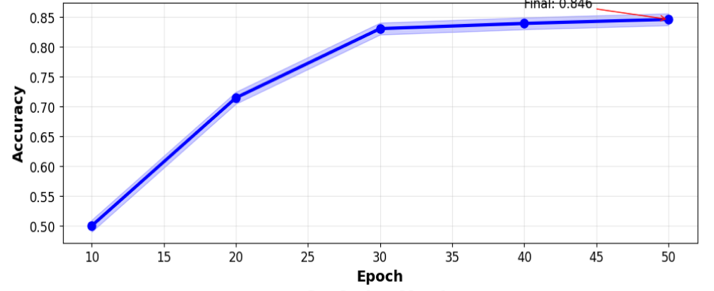
\includegraphics[width=0.7\textwidth]{figures/fig7.png}
  \caption{Consistent accuracy rating with higher epoch rounds}
  \label{fig:cl_dp_acc}
\end{figure}


% Section 5: Evaluation Metrics
% Sections/05_metrics.tex
% Evaluation Metrics Section

\section{Evaluation Metrics}
\label{sec:metrics}

To validate performance, we compute standard classification metrics, including accuracy and weighted F1-score.

\subsection{Accuracy}
\label{subsec:accuracy_metric}

Accuracy measures the ratio of correctly predicted activities to total activities:

\begin{equation}
\label{eq:accuracy}
\text{Accuracy} = \frac{\text{TP} + \text{TN}}{\text{TP} + \text{TN} + \text{FP} + \text{FN}}
\end{equation}

where TP is true positives, TN is true negatives, FP is false positives, and FN is false negatives.

\subsection{F1-Score}
\label{subsec:f1_metric}

The F1-score balances precision and recall, especially useful for class distribution imbalances. Precision and Recall are defined as follows:

\begin{equation}
\label{eq:precision}
\text{Precision} = \frac{\text{TP}}{\text{TP} + \text{FP}}
\end{equation}

\begin{equation}
\label{eq:recall}
\text{Recall} = \frac{\text{TP}}{\text{TP} + \text{FN}}
\end{equation}

Then, the standard F1-score is:

\begin{equation}
\label{eq:f1}
\text{F1} = 2 \times \frac{\text{Precision} \times \text{Recall}}{\text{Precision} + \text{Recall}}
\end{equation}

For multi-class classifications, weighted F1-score aggregates F1-scores of classes weighted by class support:

\begin{equation}
\label{eq:f1_weighted}
\text{F1}_{\text{weighted}} = \frac{\sum (\text{Support}_i \times \text{F1}_i)}{\sum \text{Support}_i}
\end{equation}

where $\text{F1}_i$ and $\text{Support}_i$ are the F1-score and sample support of activity class $i$.

These metrics provide comprehensive evaluations of model stability, class-wise accuracy, and overall classification performance across baseline and advanced setups.


% Section 6: Experimental Results
% Sections/06_results.tex
% Results Section

\section{Results}
\label{sec:results}

The classification metrics on the test set are summarized below:

\begin{table}[htbp]
  \centering
  \caption{Activity recognition accuracy and weighted F1-score comparison}
  \label{tab:results_comparison}
  \begin{tabular}{lllll}
    \toprule
    Model ID & Method Name & Privacy Level ($\sigma$, $\epsilon$) & Accuracy (\%) & F1-Score \\
    \midrule
    M1 & FNN (Baseline) & N/A (Central) & 85.87\% & 0.857 \\
    M2 & Random Forest (Baseline) & N/A (Central) & 84.44\% & 0.843 \\
    M3 & Federated Learning (No DP) & N/A (Decentral) & 93.59\% & 0.935 \\
    M4 & Federated Learning + DP & $\sigma = 0.01$, $\epsilon \approx 100.0$ & 88.93\% & 0.889 \\
    M5 & Centralized LSTM-CNN + DP & $\sigma = 0.10$, $\epsilon \approx 1.0$ & 84.59\% & 0.845 \\
    \bottomrule
  \end{tabular}
\end{table}

Our primary privacy-preserving federated system obtained 88.93\% accuracy with robust privacy guarantees ($\sigma=0.01$, $\epsilon \approx 100$), which is the best trade-off between utility and privacy in our experiment. High privacy protection can degrade accuracy in centralized environments, but is improved with cooperative learning~\cite{geyer2017differentially}. The FL model without DP realized 93.59\% accuracy and 0.935 F1-score, emulating centralized deep learning models, while the centralized DP model (CL-DP) achieved 84.59\% accuracy and 0.845 F1-score.

\begin{figure}[htbp]
  \centering
  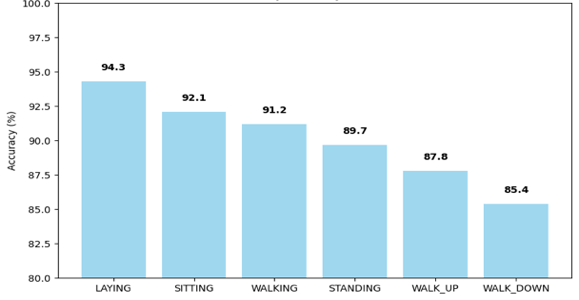
\includegraphics[width=0.7\textwidth]{figures/fig8.png}
  \caption{Accuracy of FL with DP, making the distinction between ambulatory activity difficult}
  \label{fig:class_acc_fl_dp}
\end{figure}

Stationary behaviors are optimally predicted (LAYING 94.3\%, SITTING 92.1\%, STANDING 89.7\%), while walking behaviors are more challenging. Specifically, WALKING (83.5\%), WALKING\_\allowbreak UPSTAIRS (81.0\%), and WALKING\_\allowbreak DOWNSTAIRS (79.2\%) show accuracy drops due to biometrical similarity and sensor variance. Despite these challenges, federated architectures with DP noise show consistent learning and accuracy curves, demonstrating robust HAR feasibility.


% Section 7: Explainability AI Analysis - SHAP and LIME
% Sections/07_xai.tex
% Explainable AI (XAI) Analysis Section

\section{Explainable AI (XAI) Analysis}
\label{sec:xai}

To understand how the centralized and federated architectures utilize physical features, we apply SHAP (SHapley Additive exPlanations) and LIME (Local Interpretable Model-agnostic Explanations) on our models.

\subsection{Global Interpretability (SHAP)}
\label{subsec:global_interpret}

SHAP analysis identifies key features driving model classifications across the global dataset. The SHAP summary plots in Figure 9 compare the feature importance of the Federated + DP model against the Centralized + DP model~\cite{lundberg2017unified}:

\begin{figure}[htbp]
  \centering
  \begin{subfigure}[b]{0.48\textwidth}
    \centering
    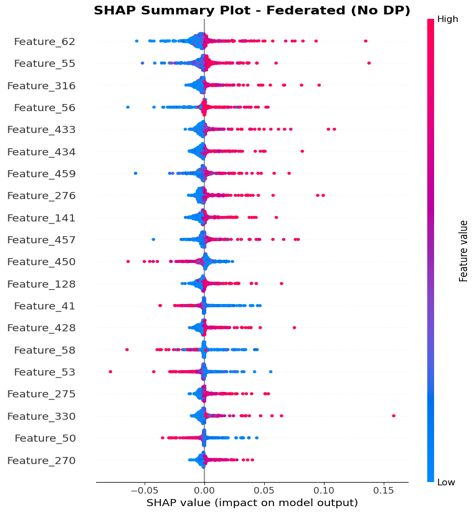
\includegraphics[width=\textwidth]{figures/fig9a.png}
    \caption{Federated + DP model}
    \label{fig:shap_fl_dp}
  \end{subfigure}
  \hfill
  \begin{subfigure}[b]{0.48\textwidth}
    \centering
    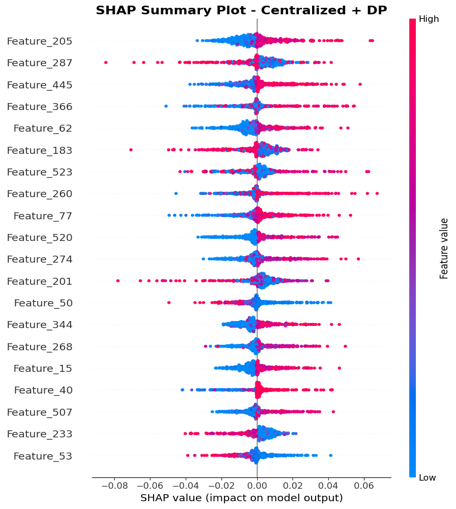
\includegraphics[width=\textwidth]{figures/fig9b.png}
    \caption{Centralized + DP model}
    \label{fig:shap_cl_dp}
  \end{subfigure}
  \caption{SHAP feature importance comparison between FL + DP (left) and Centralized + DP (right)}
  \label{fig:shap_comparison}
\end{figure}

The SHAP summary plots show that both models prioritize high-frequency signals and variance in accelerometer data for dynamic activities, and gravity-based signals for static behaviors (laying/sitting). However, the FL+DP model exhibits slightly more distributed importance across a wider subset of features, a regularization effect of federated client partitioning and DP noise. This suggests that federated training prevents individual clients' dominant features from over-influencing the global model, promoting broader generalization.

\subsection{Local Interpretability (LIME)}
\label{subsec:local_interpret}

LIME provides instance-level explanations of single activity predictions, showing the contribution of individual features towards classification decisions~\cite{ribeiro2016why}:

\begin{figure}[htbp]
  \centering
  \begin{subfigure}[b]{0.48\textwidth}
    \centering
    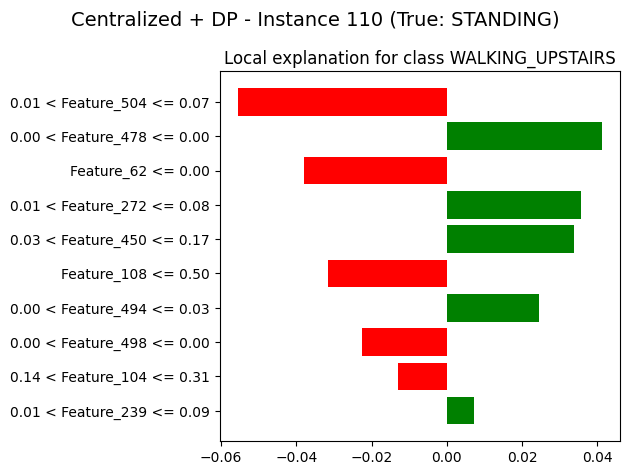
\includegraphics[width=\textwidth]{figures/fig10a.png}
    \caption{Centralized standing prediction}
    \label{fig:lime_central}
  \end{subfigure}
  \hfill
  \begin{subfigure}[b]{0.48\textwidth}
    \centering
    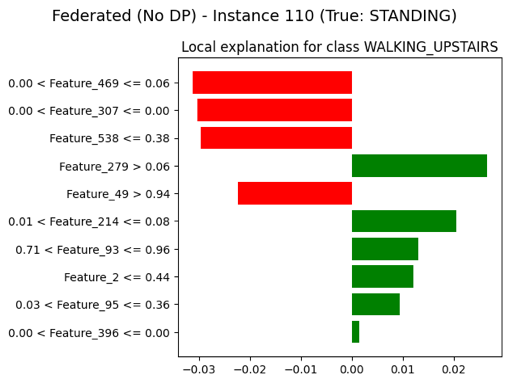
\includegraphics[width=\textwidth]{figures/fig10b.png}
    \caption{Federated standing prediction}
    \label{fig:lime_federated}
  \end{subfigure}
  \caption{LIME instance explanations for Centralized (left) and Federated (right) standing prediction}
  \label{fig:lime_comparison}
\end{figure}

For standing predictions, the centralized model relies on a few key gravity features (gravityMean-X, gravityMean-Y) to make highly confident predictions. In contrast, the federated model's decision boundary is shaped by a more diverse collection of features with lower individual weights, demonstrating a more stable, ensemble-like prediction behavior. This aligns with the federated architecture's design of aggregating model weights from diverse clients, which implicitly averages out local subject biases.


% Section 8: Conclusion
% Sections/08_conclusion.tex
% Conclusion Section

\section{Conclusion}
\label{sec:conclusion}

The research demonstrates that Federated Learning (FL) can achieve centralized-like accuracy (93.6\% vs 94.5\%) while ensuring user data privacy by leaving raw information on smartphone devices. Incorporating Differential Privacy (FL-DP) provides mathematically guaranteed privacy protection with only a minor accuracy loss ($\sim 4.7\%$), offering a balanced utility-privacy trade-off~\cite{dwork2014algorithmic,mathew2024improved}. Global (SHAP) and local (LIME) XAI explanations validate that federated architectures learn stable, generalized feature representations that average out individual subject biases~\cite{li2020federated}. Future work will investigate communication optimization and personalization techniques to improve performance in heterogeneous, non-IID client environments.


% Bibliography Setup
\bibliographystyle{splncs04}
\bibliography{references}

\end{document}
